\documentclass[12pt]{article}

\usepackage{sbc-template}
\usepackage{graphicx,url}
\usepackage[brazil]{babel}
\usepackage[utf8]{inputenc}
\usepackage{amsmath}
\usepackage{booktabs}
\usepackage{float}
\usepackage{placeins}
\usepackage{enumitem}
\usepackage{tikz}
\usepackage{microtype}
\usepackage[hidelinks]{hyperref}

\setlength{\textfloatsep}{5pt plus 1pt minus 2pt}
\setlength{\floatsep}{5pt plus 1pt minus 2pt}
\setlength{\intextsep}{5pt plus 1pt minus 2pt}
\setlength{\abovecaptionskip}{3pt}
\setlength{\belowcaptionskip}{2pt}
\setlist{nosep}

\sloppy

\title{Uma solução para o Problema de Roteamento de Veículos Capacitado utilizando GRASP e GRASP Reativo}

\author{João Vitor Soares dos Santos\inst{1}, Pedro Henrique de Castro Cunha Quedevez\inst{1}}

\address{Curso de Ciência da Computação -- Universidade Federal do Espírito Santo (UFES)\\
Vitória -- ES -- Brasil}

\begin{document}

\maketitle

\begin{abstract}
This article presents an experimental study of the Capacitated Vehicle Routing Problem (CVRP) using the Greedy Randomized Adaptive Search Procedure (GRASP) and its reactive variant. The solution combines randomized greedy construction, Restricted Candidate Lists (RCL), and best-improvement local search. Instances A and B from the CVRPLIB/Augerat benchmark set were solved five times for both methods. Parameter calibration selected $\alpha=0.25$ from $0.25$, $0.50$, and $0.75$. Across 50 instance-method experiments, Reactive GRASP obtained an average gap of $17.24\%$, against $17.63\%$ for classical GRASP. The reactive approach was also slower on average. These results indicate that Reactive GRASP can improve average quality, but does not consistently dominate the calibrated classical method.
\end{abstract}

\begin{resumo}
Este artigo apresenta um estudo experimental do Problema de Roteamento de Veículos Capacitado (CVRP) com o Greedy Randomized Adaptive Search Procedure (GRASP) e sua versão reativa. A solução combina construção gulosa aleatorizada, Lista Restrita de Candidatos (RCL) e busca local do tipo melhor melhora. Foram resolvidas cinco vezes todas as instâncias dos conjuntos A e B da biblioteca Augerat. Na calibração, $\alpha=0.25$ apresentou o menor gap médio dentre $0.25$, $0.50$ e $0.75$. Considerando as 50 combinações instância--método, o GRASP Reativo obteve gap médio de $17.24\%$, contra $17.63\%$ do GRASP clássico. Os resultados mostram melhoria média no reativo, mas não dominância consistente sobre o GRASP clássico calibrado.
\end{resumo}

\section{Introdução}

O Problema de Roteamento de Veículos (Vehicle Routing Problem -- VRP) surgiu no contexto da programação de entregas e da organização de frotas \cite{dantzig1959}. No Problema de Roteamento de Veículos Capacitado (Capacitated Vehicle Routing Problem -- CVRP), existe um depósito, um conjunto de clientes com demandas conhecidas e uma frota de veículos com capacidade limitada. Cada cliente deve ser atendido exatamente uma vez, todas as rotas começam e terminam no depósito, e a carga de cada veículo não pode exceder sua capacidade. O objetivo é minimizar a distância total percorrida.

O CVRP é um problema de otimização combinatória de difícil resolução, pois o número de sequências viáveis cresce rapidamente com a quantidade de clientes. Meta-heurísticas permitem obter soluções de boa qualidade em tempo limitado. O GRASP (Greedy Randomized Adaptive Search Procedure) combina construção gulosa aleatorizada com busca local \cite{feo1989,resende2019}.

Este trabalho compara o GRASP clássico, com $\alpha$ fixo, ao GRASP Reativo, que adapta a distribuição de probabilidades dos valores de $\alpha$ durante a execução. Foram usadas 53 instâncias dos conjuntos A (27), B (23) e F (3), da biblioteca CVRPLIB. Os conjuntos A e B são de Augerat; o nome indica a dimensão e a frota, como em \texttt{A-n32-k5} (32 nós e 5 veículos). Cada arquivo traz coordenadas bidimensionais, demandas, depósito, capacidade e, quando informado, o valor ótimo conhecido, usado para calcular o gap. As distâncias seguem \texttt{EUC\_2D}, arredondadas ao inteiro mais próximo:
\begin{equation}
d_{ij}=\left\lfloor\sqrt{(x_i-x_j)^2+(y_i-y_j)^2}+0.5\right\rfloor.
\end{equation}

\section{Representação de uma solução}

Uma solução $S=(R_1,\ldots,R_k)$ é uma lista de rotas, em que cada posição $j$ da lista corresponde a um caminhão (veículo) e $R_j$ é a rota que ele percorre, uma lista ordenada de clientes, $R=(v_1,\ldots,v_m)$. O depósito (nó $0$) não é armazenado: ele é implícito no início e no fim, de modo que a rota percorrida é $0\rightarrow v_1\rightarrow\cdots\rightarrow v_m\rightarrow 0$. Rotas vazias são descartadas, e o número de rotas não pode exceder o número de veículos da instância, obtido do sufixo \texttt{-k} do nome do arquivo.

Uma solução é \emph{viável} quando atende todos os clientes exatamente uma vez, usa no máximo $k$ rotas e respeita a capacidade em cada rota. Essa verificação é independente do custo: uma solução de custo baixo pode ser inválida se omitir ou repetir um cliente, ou exceder a capacidade. Por isso toda solução é validada antes de ser aceita como melhor solução.

\textbf{Exemplo.} Solução obtida pelo GRASP clássico ($\alpha=0.25$, 100 iterações, semente 42) na instância \texttt{A-n32-k5} (31 clientes, 5 veículos, capacidade 100; no arquivo, o depósito é o nó 1). Seu custo é 808, com gap de 3.06\% em relação ao ótimo conhecido (784):
{\small
\begin{align*}
S=\big(&[25,28],\ [21,6,30,19,12,5,24,4,3,7],\ [15,29,9,10,23,16,11,26],\\
&[31,17,2,13],\ [22,32,20,18,14,8,27]\big).
\end{align*}}
Cada posição da lista $S$ corresponde a um caminhão: o primeiro caminhão atende os clientes $[25,28]$, o segundo atende $[21,6,30,\ldots,7]$, e assim por diante, totalizando os 5 veículos da instância. Dentro de cada rota, a ordem dos clientes é a ordem de visita. As cargas dos caminhões são 44, 98, 98, 72 e 98, todas dentro da capacidade, e cada um dos 31 clientes aparece uma única vez. A primeira rota, por exemplo, percorre $\text{depósito}\rightarrow 25\rightarrow 28\rightarrow\text{depósito}$.

O custo de uma rota é
\begin{equation}
C(R)=d_{0v_1}+\sum_{i=1}^{m-1}d_{v_iv_{i+1}}+d_{v_m0},
\end{equation}
e a função objetivo, a ser minimizada, é $F(S)=\sum_{j=1}^{k}C(R_j)$. O gap em relação ao ótimo conhecido $F^*$ é
\begin{equation}
\text{gap}(S)=100\left(\frac{F(S)}{F^*}-1\right).
\end{equation}
A matriz de distâncias é calculada uma vez por instância e reutilizada na construção, na validação e nos movimentos da busca local.

\section{Descrição geral do algoritmo}

O GRASP segue um ciclo multi-start (Figura~\ref{fig:pseudogeral}): em cada iteração, constrói-se uma solução viável por um procedimento guloso aleatorizado, repara-se a solução caso ela seja inviável, aplica-se a busca local e atualiza-se a melhor solução global. As iterações são independentes entre si. O critério de parada é o número máximo de iterações (100 nos experimentos finais).

\begin{figure}[H]
\centering
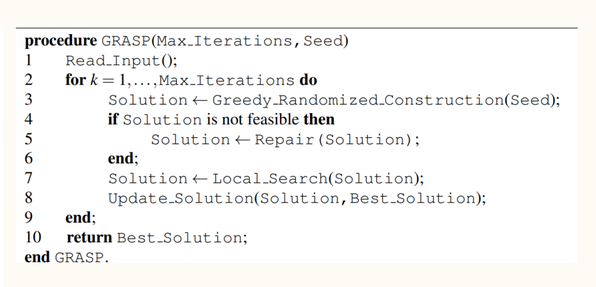
\includegraphics[width=0.50\textwidth]{imagens/pseudo-codigo-geral.png}
\caption{Pseudocódigo geral do GRASP adaptado à implementação.}
\label{fig:pseudogeral}
\end{figure}

No GRASP clássico, o parâmetro $\alpha$ da lista restrita de candidatos (RCL) permanece constante. No GRASP Reativo, $\alpha$ é sorteado a cada iteração dentre uma grade $\mathcal{A}$ de valores ($0$ a $1$, com passo $0.05$, totalizando 21 valores). Inicialmente, cada valor de $\mathcal{A}$ é usado uma vez, e o custo obtido passa a ser seu custo médio $\bar F(\alpha)$. A cada bloco de 2 iterações, $\bar F(\alpha)$ é recalculado com as soluções do bloco, e a probabilidade de escolher $\alpha$ passa a ser
\begin{equation}
p(\alpha)=
\frac{\left(F_{\mathrm{melhor}}/\bar F(\alpha)\right)^\delta}
{\displaystyle\sum_{\beta\in\mathcal{A}}
\left(F_{\mathrm{melhor}}/\bar F(\beta)\right)^\delta},
\end{equation}
em que $F_{\mathrm{melhor}}$ é o menor custo encontrado até então. A normalização faz as probabilidades somarem 1, e $\delta=5$ controla a preferência por valores de $\alpha$ com bom desempenho: quanto maior $\delta$, mais forte a preferência. O ótimo conhecido da instância não é usado nesse cálculo. No reativo, as 21 avaliações iniciais contam entre as 100 do orçamento, de modo que os dois métodos avaliam o mesmo número de soluções.

O $\alpha$ do GRASP clássico é escolhido antes dos experimentos finais, por calibração (Seção~\ref{sec:experimentos}).

\section{Descrição geral dos algoritmos}

O GRASP segue um ciclo multi-start ilustrado pela Figura~\ref{fig:pseudogeral}. Em cada iteração, constrói-se uma solução viável, executa-se a busca local e atualiza-se a melhor solução global.

\begin{figure}[H]
\centering
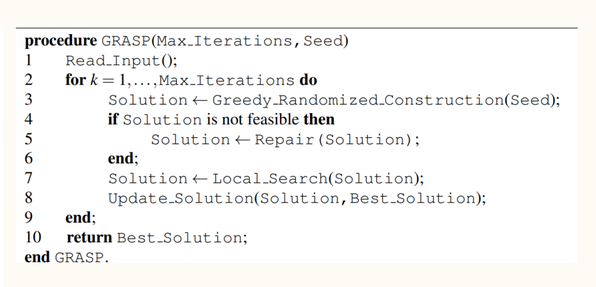
\includegraphics[width=0.72\textwidth]{imagens/pseudo-codigo-geral.png}
\caption{Pseudocódigo geral do GRASP adaptado à implementação.}
\label{fig:pseudogeral}
\end{figure}

A construção produz diversidade e a busca local intensifica a solução. No GRASP clássico, $\alpha$ permanece constante. No GRASP Reativo, as probabilidades de escolha dos valores de $\alpha$ são atualizadas ao fim de cada bloco, com base nos custos observados. A probabilidade de escolher um valor $\alpha$ é calculada por
\begin{equation}
p(\alpha)=
\frac{\left(F_{\mathrm{melhor}}/\bar F(\alpha)\right)^\delta}
{\displaystyle\sum_{\beta\in\mathcal{A}}
\left(F_{\mathrm{melhor}}/\bar F(\beta)\right)^\delta},
\end{equation}
em que $\bar F(\alpha)$ é o custo médio das soluções obtidas com $\alpha$, $F_{\mathrm{melhor}}$ é o menor custo encontrado até então e $\mathcal{A}$ é o conjunto de valores de $\alpha$. A normalização faz com que as probabilidades somem 1. O parâmetro $\delta=5$ controla a preferência por valores de $\alpha$ com melhor desempenho: quanto maior $\delta$, maior essa preferência. O ótimo conhecido da instância não é usado nesse cálculo.

A calibração seleciona um único $\alpha$ antes dos experimentos finais usando instâncias representativas. O GRASP Reativo, por sua vez, atualiza as probabilidades de uma grade de valores durante a execução.
\section{Algoritmo construtivo}

A construção prioriza clientes com maiores demandas. Para o cliente escolhido, avaliam-se as posições viáveis nas rotas. O custo incremental de uma inserção é
\[
\Delta=C(R^{p,v})-C(R).
\]
Os candidatos formam a RCL definida por
\begin{equation}
\Delta \leq c_{min}+\alpha(c_{max}-c_{min}),
\end{equation}
e uma posição é sorteada nessa lista.

Assim, $\alpha=0$ admite apenas o melhor incremento, $\alpha=1$ aceita todos os candidatos viáveis e valores intermediários equilibram guloseima e aleatoriedade. Os custos são recalculados após cada inserção. Quando não há candidato viável, uma busca limitada por backtracking distribui os clientes restantes.

\begin{figure}[H]
\centering
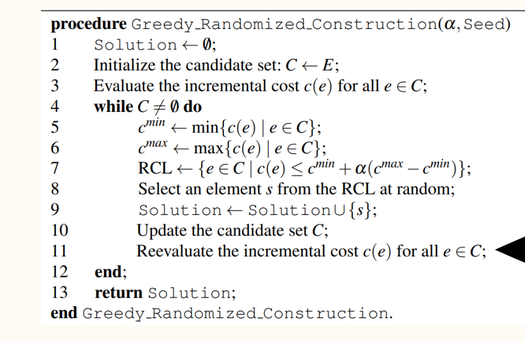
\includegraphics[width=0.72\textwidth]{imagens/pseudo-codigo-construcao.png}
\caption{Pseudocódigo da construção gulosa aleatorizada.}
\label{fig:pseudoconstrucao}
\end{figure}

\section{Busca local}

A busca local utiliza a estratégia \textit{best-improvement}. Ela avalia 2-opt, realocação e troca entre rotas. Movimentos que excedem a capacidade são descartados.

Em cada iteração, avalia todas as vizinhanças, aplica o movimento com maior redução $\Delta C<0$ e repete o processo até não existir melhora ou atingir 20 movimentos nos experimentos. A variante \textit{first-improvement}, apesar de implementada, não participa dos experimentos.

A implementação foi desenvolvida em Python 3.9.12. Os experimentos foram executados em um processador Intel Core i7-8565U, com oito CPUs disponíveis. Os dados das instâncias e as soluções são armazenados em listas e dicionários de Python.

\section{Calibração dos hiperparâmetros}

A calibração comparou $\alpha\in\{0.25,0.50,0.75\}$ nas instâncias \texttt{A-n32-k5}, \texttt{A-n80-k10} e \texttt{B-n78-k10}. Para cada combinação instância--$\alpha$, foram realizadas cinco execuções independentes, com sementes reproduzíveis. O limite foi de 50 iterações, 20 movimentos máximos de busca local e 180 segundos por execução.

A escolha considerou a média dos gaps obtidos nas três instâncias. Em caso de empate, seria utilizado o custo médio agregado.

\begin{table}[htbp]
\centering
\caption{Resumo da calibração manual do parâmetro $\alpha$.}
\label{tab:calibracao}
\small
\begin{tabular}{lrrrrrr}
\toprule
Instância & Ótimo & $\alpha$ & Custo mín. & Custo méd. & Gap mín. & Gap méd. \\
\midrule
A-n32-k5 & 784 & 0.25 & 808 & 826.4 & 3.06\% & 5.41\% \\
A-n32-k5 & 784 & 0.50 & 816 & 832.0 & 4.08\% & 6.12\% \\
A-n32-k5 & 784 & 0.75 & 819 & 838.4 & 4.46\% & 6.94\% \\
A-n80-k10 & 1763 & 0.25 & 2180 & 2195.8 & 23.65\% & 24.55\% \\
A-n80-k10 & 1763 & 0.50 & 2142 & 2195.4 & 21.50\% & 24.53\% \\
A-n80-k10 & 1763 & 0.75 & 2176 & 2213.0 & 23.43\% & 25.52\% \\
B-n78-k10 & 1221 & 0.25 & 1668 & 1687.4 & 36.61\% & 38.20\% \\
B-n78-k10 & 1221 & 0.50 & 1685 & 1697.4 & 38.00\% & 39.02\% \\
B-n78-k10 & 1221 & 0.75 & 1644 & 1678.6 & 34.64\% & 37.48\% \\
\bottomrule
\end{tabular}
\end{table}

Os gaps médios agregados por $\alpha$ foram aproximadamente 22.72\% para 0.25, 23.22\% para 0.50 e 23.31\% para 0.75. Assim, $\alpha=0.25$ foi selecionado para o GRASP clássico nos experimentos finais.

\section{Experimentos e resultados}

Os experimentos finais utilizam as instâncias dos conjuntos A, B e F disponíveis no diretório \texttt{instancias}. O GRASP clássico foi configurado com $\alpha=0.25$, 50 iterações e 20 movimentos locais. O GRASP Reativo utilizou uma grade de $\alpha$ com passo $0.05$, bloco de atualização igual a 2 e $\delta=5$.

Os dois métodos foram executados cinco vezes em cada instância. Foram registrados custo mínimo, custo médio, tempo mínimo, tempo médio e gaps. A agregação apresentou gap mínimo médio de 14.79\% no clássico e 14.29\% no reativo; os gaps médios foram 17.63\% e 17.24\%. O tempo médio foi 4.23 s no clássico e 6.05 s no reativo.

Considerando as cinco execuções de cada uma das 50 instâncias, o tempo agregado aproximado foi de 1057.86 s (17 min 38 s) para o GRASP clássico e 1513.44 s (25 min 13 s) para o GRASP Reativo. Os resultados completos das cinco execuções de ambos os métodos estão disponíveis no \href{https://drive.google.com/drive/folders/1VtNmJa1JuUNSUU0BtCh_EowPccevDMAs?usp=sharing}{Drive\textsuperscript{2}}. O código, os experimentos e o notebook Jupyter estão disponíveis no \href{https://github.com/joaosoaressantos22/meta_heuristicas.git}{GitHub\textsuperscript{3}}.

\begin{table}[htbp]
\centering
\caption{Resultados finais das instâncias utilizadas na análise de convergência e TTT.}
\label{tab:destaques}
\small
\begin{tabular}{llrrrrr}
\toprule
Instância & Método & Ótimo & Mínimo & Médio & Gap mín. & Gap méd. \\
\midrule
A-n33-k5 & GRASP $\alpha=0.25$ & 661 & 670 & 687.2 & 1.36\% & 3.96\% \\
A-n33-k5 & Reactive GRASP & 661 & 669 & 677.6 & 1.21\% & 2.51\% \\
B-n31-k5 & GRASP $\alpha=0.25$ & 672 & 675 & 680.8 & 0.45\% & 1.31\% \\
B-n31-k5 & Reactive GRASP & 672 & 677 & 679.0 & 0.74\% & 1.04\% \\
\bottomrule
\end{tabular}
\end{table}

Em A-n33-k5, o reativo obteve melhor custo mínimo e médio. Em B-n31-k5, o clássico obteve melhor custo mínimo, mas o reativo obteve melhor custo médio.

\begin{figure}[htbp]
\centering
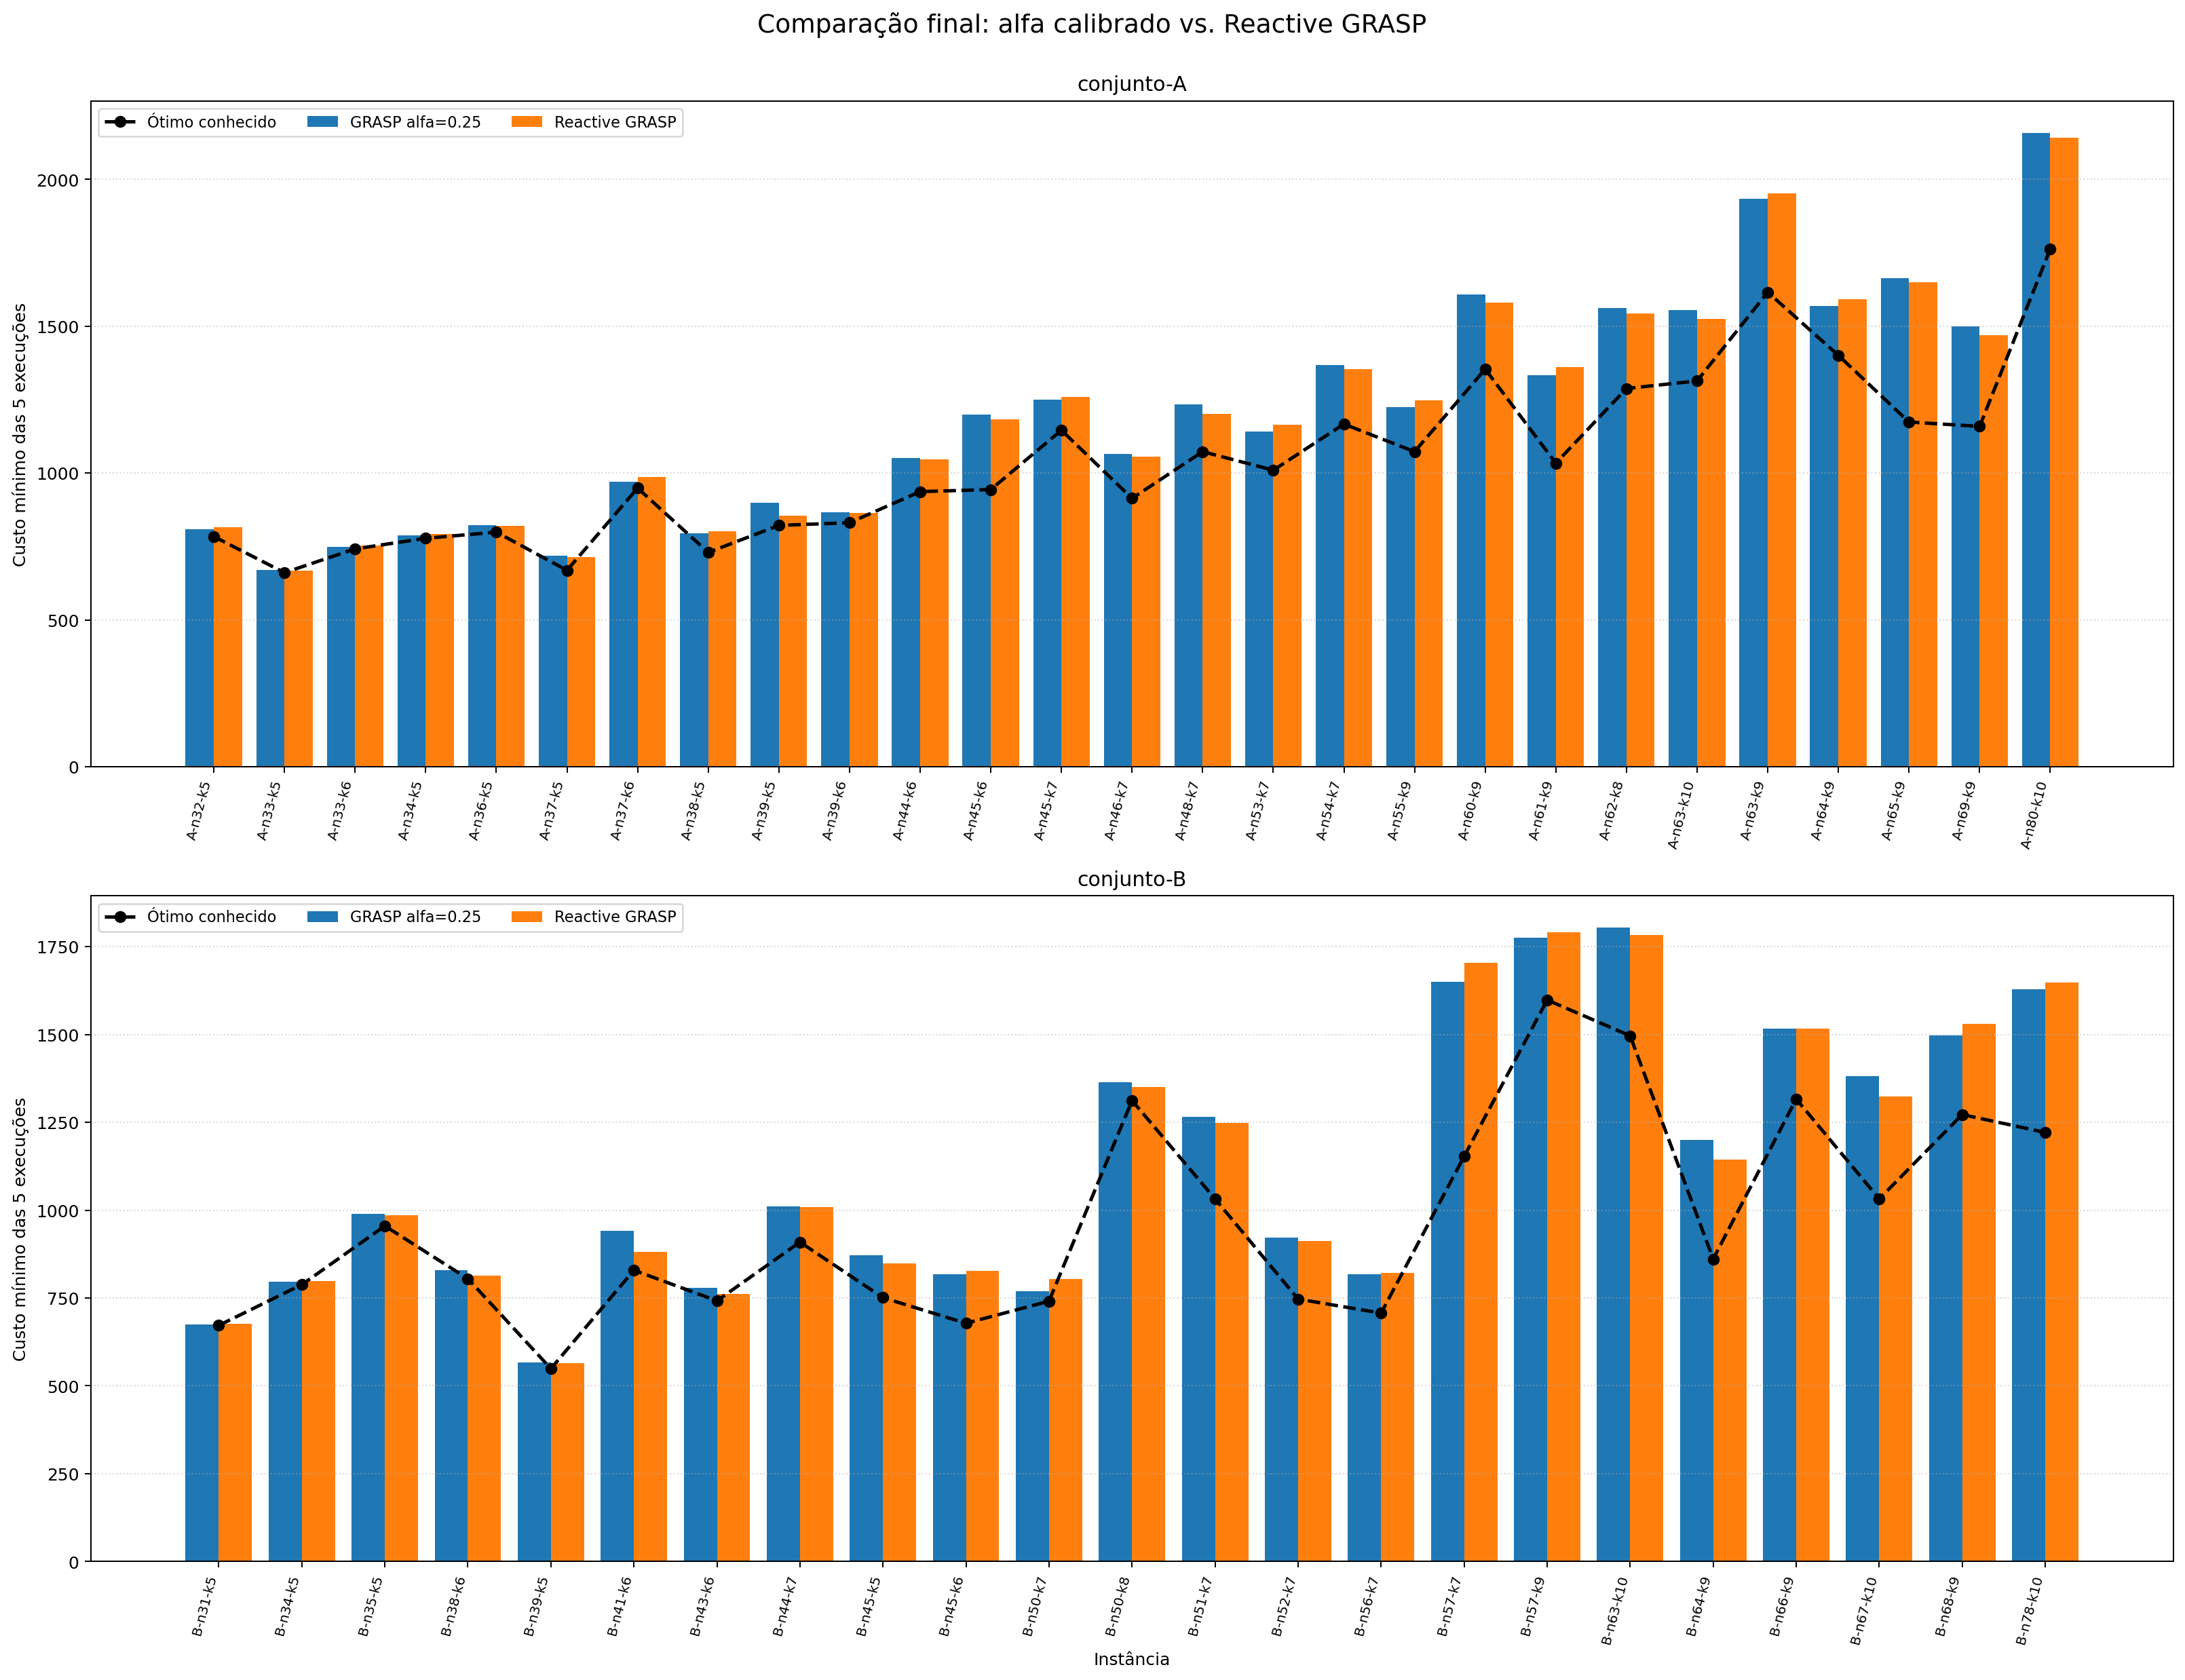
\includegraphics[width=0.90\textwidth]{imagens/comparacao_final_grasp.png}
\caption{Comparação dos custos mínimos do GRASP clássico calibrado e do GRASP Reativo.}
\label{fig:comparacao}
\end{figure}

Os gráficos de convergência mostram o melhor custo após cada solução construída e melhorada. O TTT considera o tempo até o primeiro registro igual ao ótimo conhecido; sua construção segue a abordagem de Aiex, Resende e Ribeiro \cite{aiex2007}.

\begin{figure}[htbp]
\centering
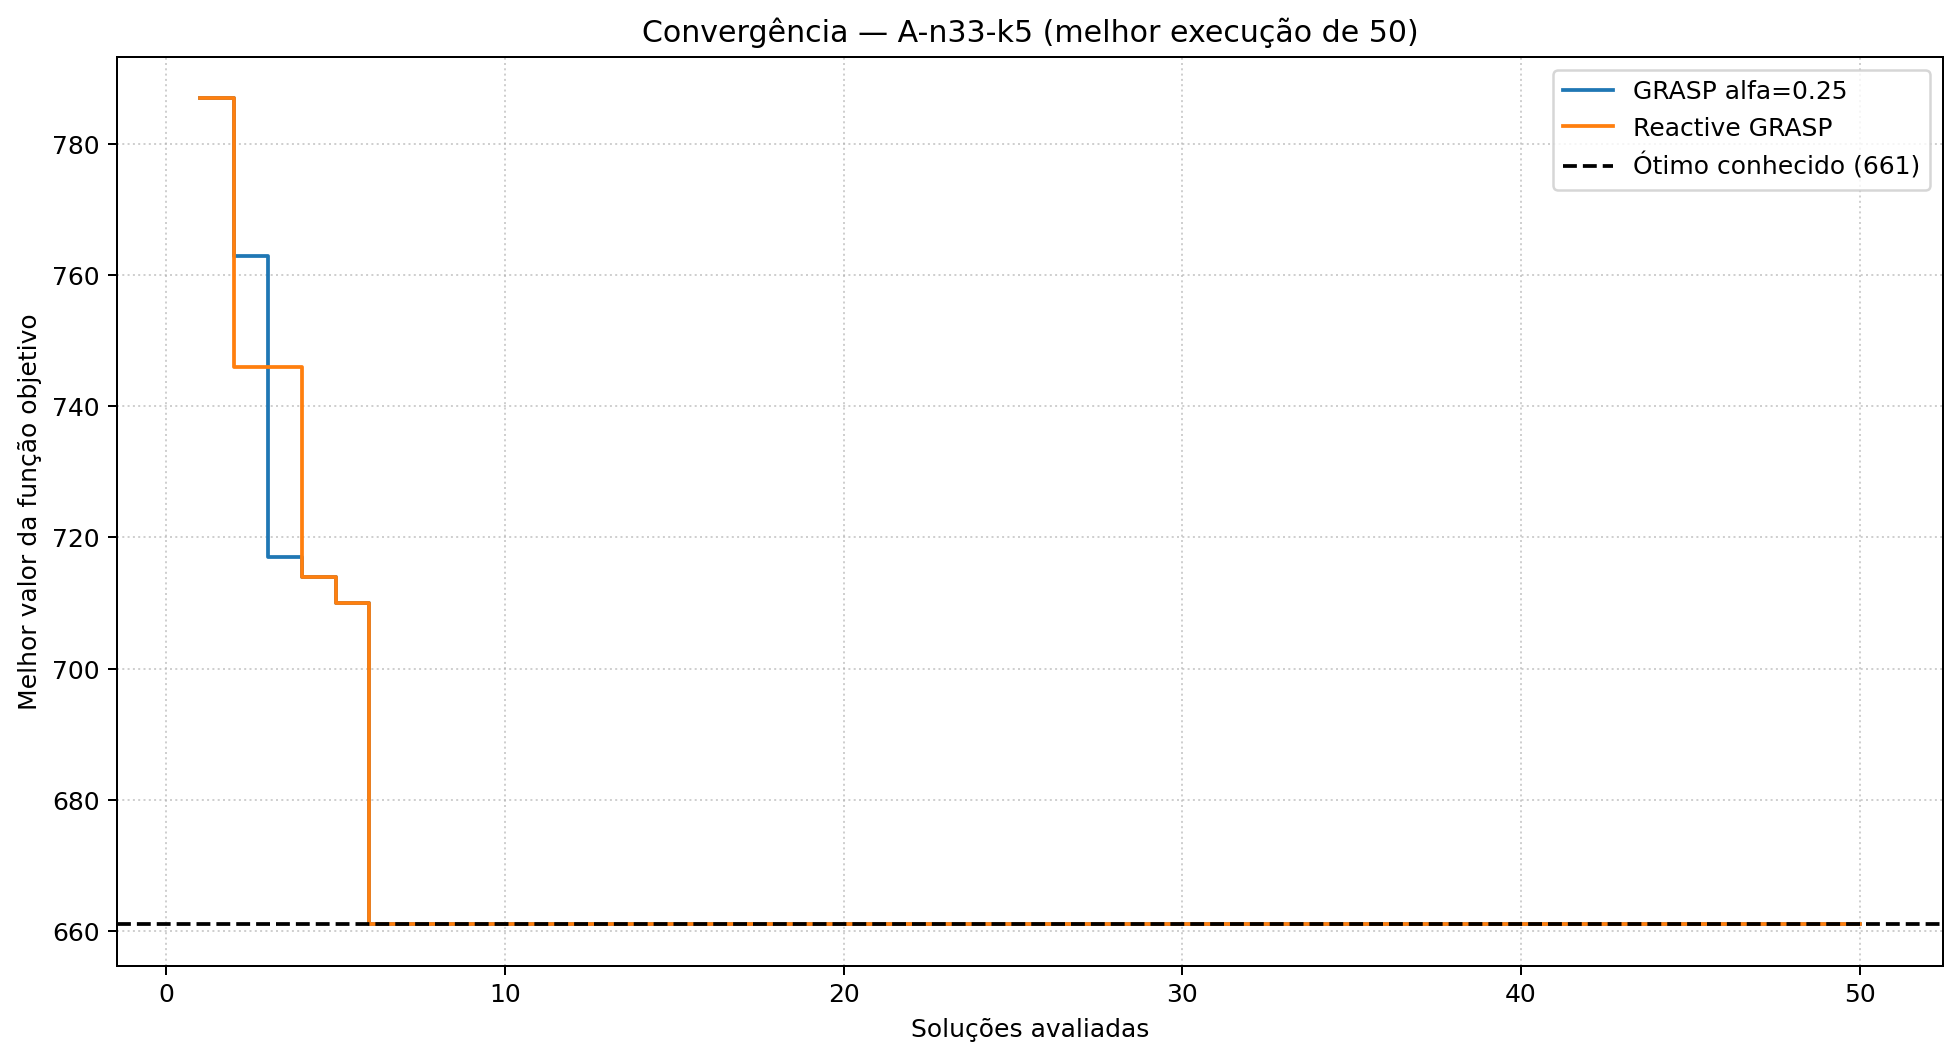
\includegraphics[width=0.98\textwidth]{imagens/convergencia_A-n33-k5.png}
\caption{Convergência em A-n33-k5.}
\label{fig:convergenciaA}
\end{figure}

\begin{figure}[htbp]
\centering
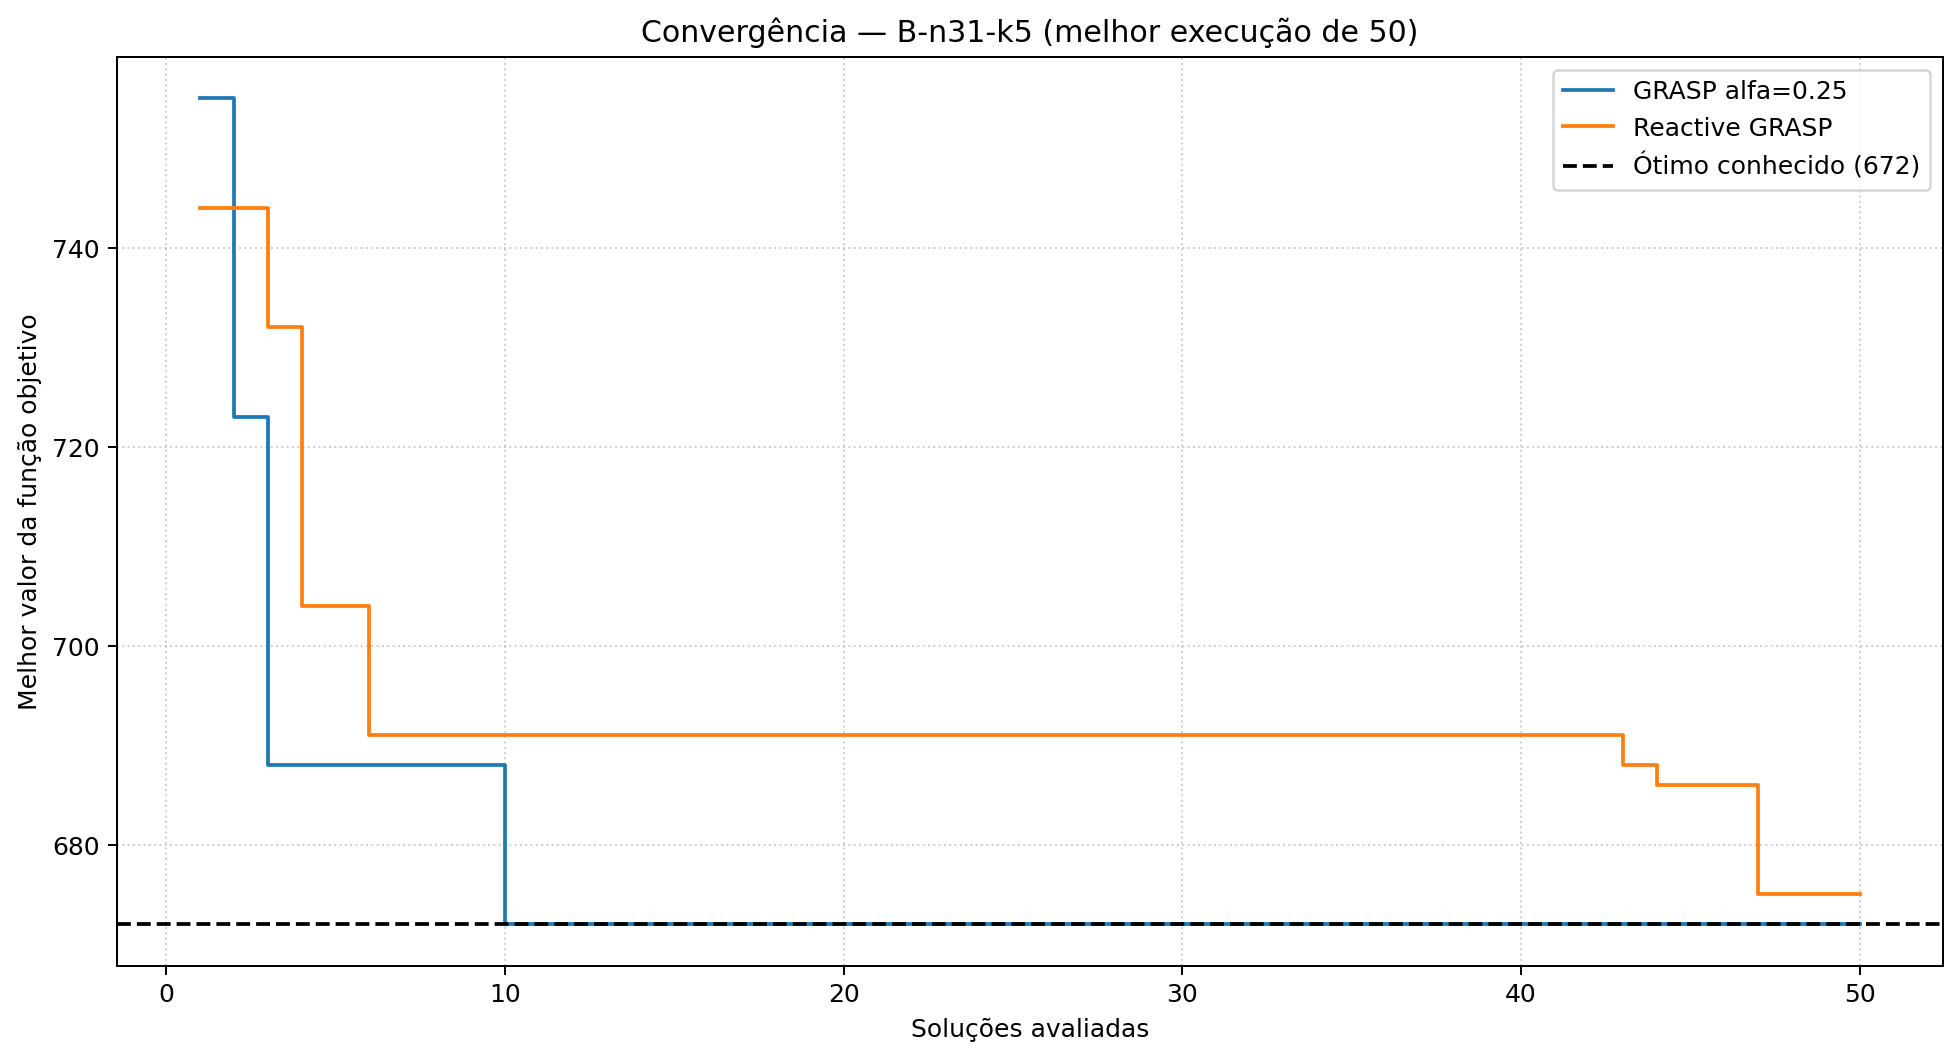
\includegraphics[width=0.98\textwidth]{imagens/convergencia_B-n31-k5.png}
\caption{Convergência em B-n31-k5.}
\label{fig:convergenciaB}
\end{figure}

Nas duas instâncias, o custo decresce rapidamente nas primeiras avaliações. Em A-n33-k5, o clássico atingiu o ótimo em duas das 50 execuções e o reativo em uma. Em B-n31-k5, o clássico encontrou o ótimo uma vez e o reativo nenhuma vez.

\begin{figure}[htbp]
\centering
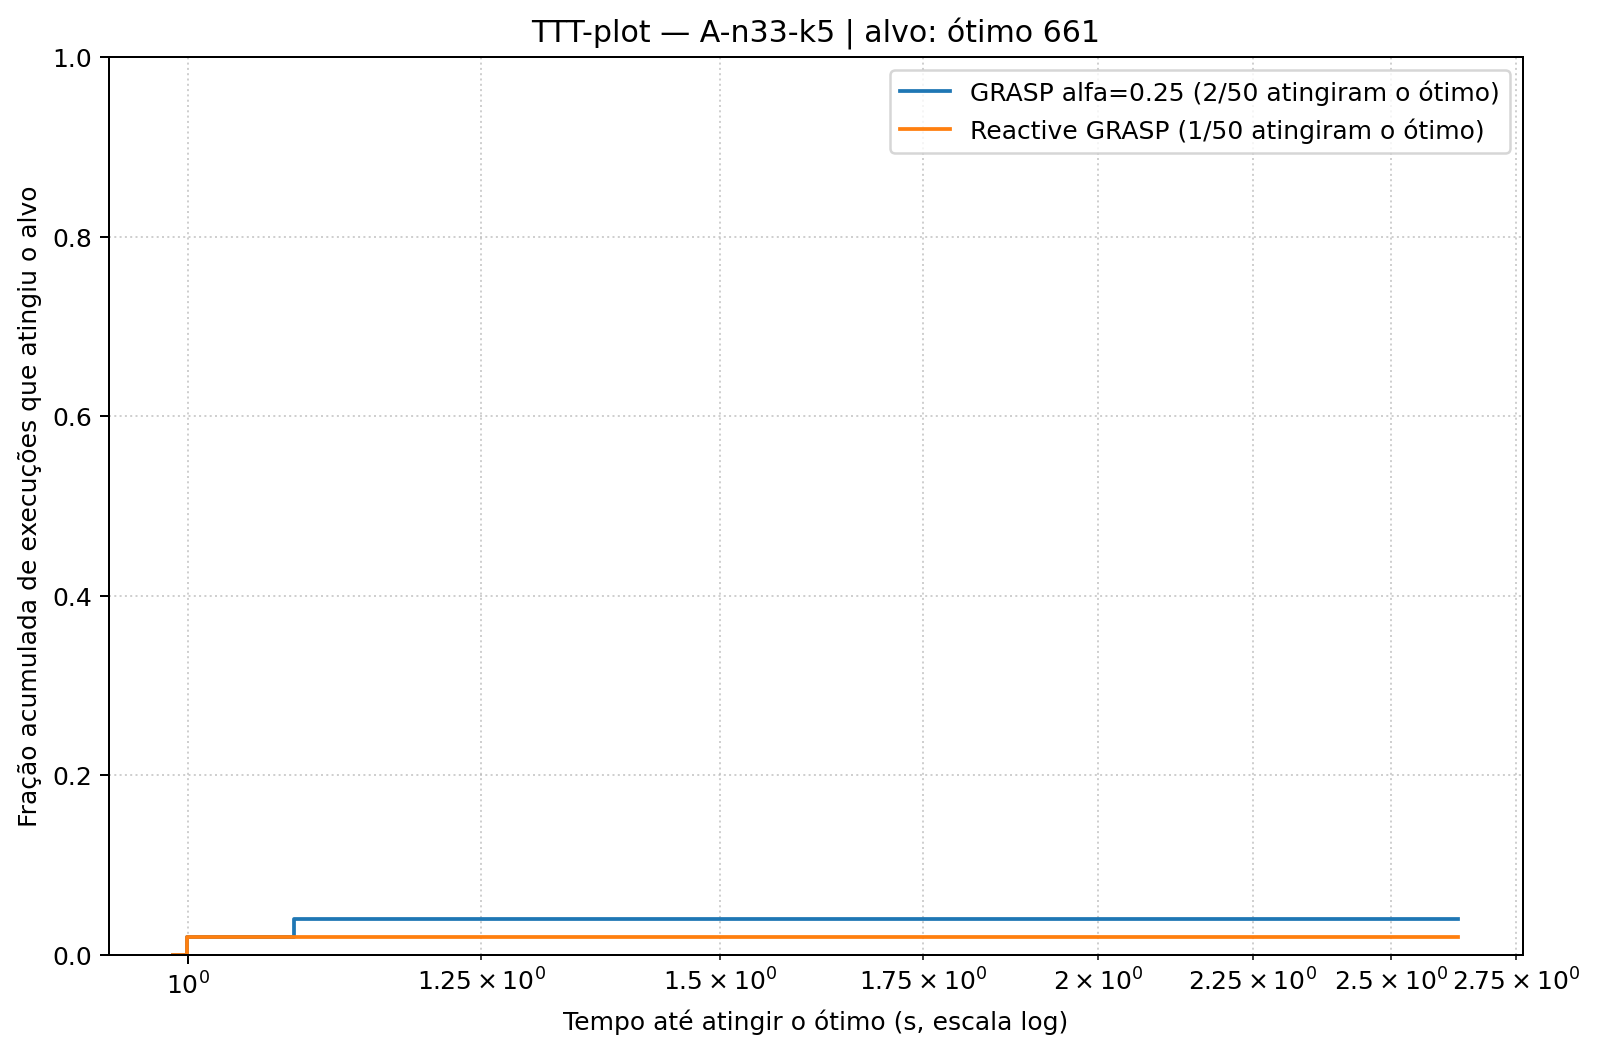
\includegraphics[width=0.98\textwidth]{imagens/ttt_A-n33-k5.png}
\caption{TTT em A-n33-k5.}
\label{fig:tttA}
\end{figure}

\begin{figure}[htbp]
\centering
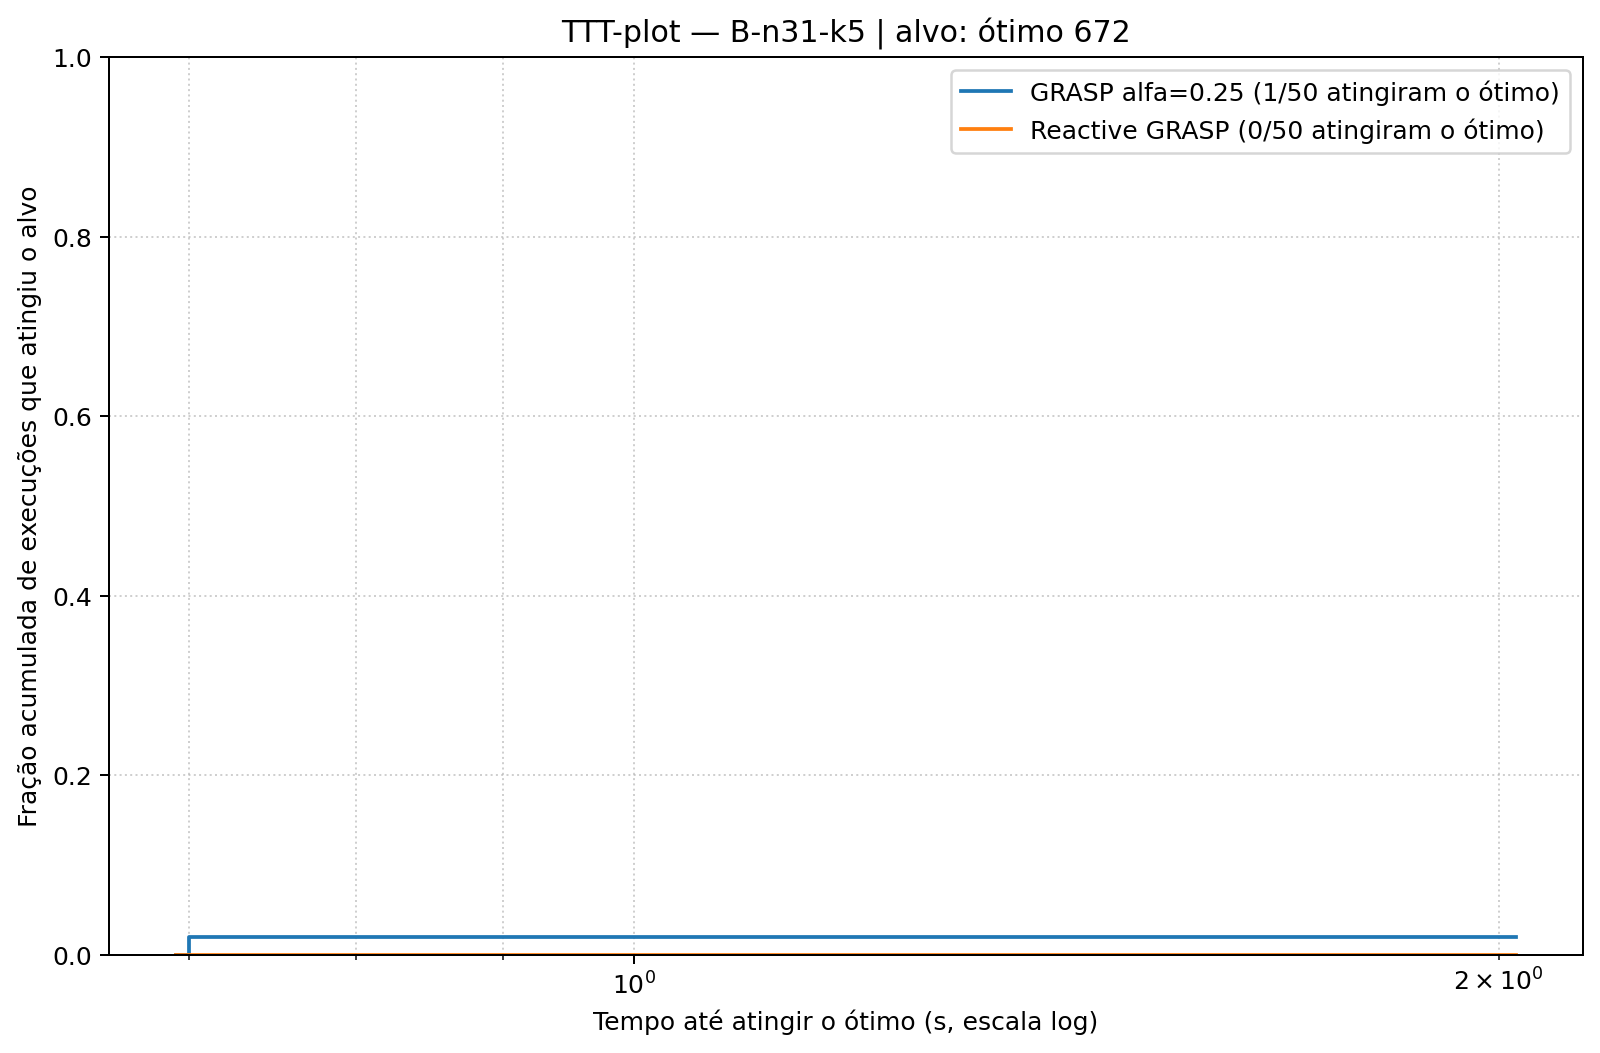
\includegraphics[width=0.98\textwidth]{imagens/ttt_B-n31-k5.png}
\caption{TTT em B-n31-k5.}
\label{fig:tttB}
\end{figure}

Em A-n33-k5, o tempo médio até o alvo foi cerca de 0.695 s no clássico e 0.280 s no reativo. Em B-n31-k5, somente o clássico encontrou o alvo, após cerca de 0.297 s. Como cada instância foi executada cinco vezes no experimento agregado, o mínimo representa o melhor resultado e a média representa a estabilidade observada.

\section{Conclusão}

O trabalho implementou e comparou o GRASP clássico e o reativo para o CVRP. A calibração selecionou $\alpha=0.25$. Nos experimentos finais, o reativo obteve gaps agregados ligeiramente menores, mas executou cerca de 43\% mais lentamente. Os gráficos não mostraram dominância: o clássico obteve mais sucessos em alcançar o ótimo em A-n33-k5 e B-n31-k5.

Como trabalhos futuros, recomenda-se ampliar as repetições e testar vizinhanças maiores ou path-relinking.


\renewcommand{\refname}{Referências}
\begingroup
\scriptsize
\bibliographystyle{sbc}
\bibliography{references}
\normalsize
\endgroup

\end{document}
